\chapter{Fragebogen}
\label{app:Fragebogen}


Dieser Abschnitt demonstriert -- als Beispiel -- die Einbindung eines externen PDF-Dokuments
in das eigene \latex-Manuskript.
Dieses Problem stellt sich relativ häufig im Zusammenhang mit Fragebögen, die
man für seine Arbeit erstellt und/oder verwendet hat, daher ist genau dieser Fall hier gezeigt.%
\footnote{Mit einem schönen Fragebogen des OÖ Energiesparverbands (\url{http://www.energiesparverband.at}).}
Wichtig ist dabei, dass die \emph{Seitenformatierung} des Dokuments intakt bleibt 
und die fortlaufende \emph{Seitennummerierung} die eingefügten Fremdseiten korrekt berücksichtigt.

\section{Das \texttt{pdfpages}-Paket}

Das \latex-Paket \texttt{pdfpages}%
\footnote{\url{https://ctan.org/pkg/pdfpages}}
ist dafür die (zurzeit) einzige Wahl und es wird mit 
%
\begin{LaTeXCode}[numbers=none]
\RequirePackage{pdfpages}
\end{LaTeXCode}
%
in der Datei \nolinkurl{hgb.sty} automatisch geladen.
Das eingebundene PDF-Dokument (der zweiseitige Frage\-bogen) liegt in
\nolinkurl{images/fragebogen.pdf}.
Um nachfolgend alle (2) Seiten der PDF-Datei in das aktuelle Dokument einzubinden,
verwenden wir die Anweisung  
%
\begin{LaTeXCode}[numbers=none]
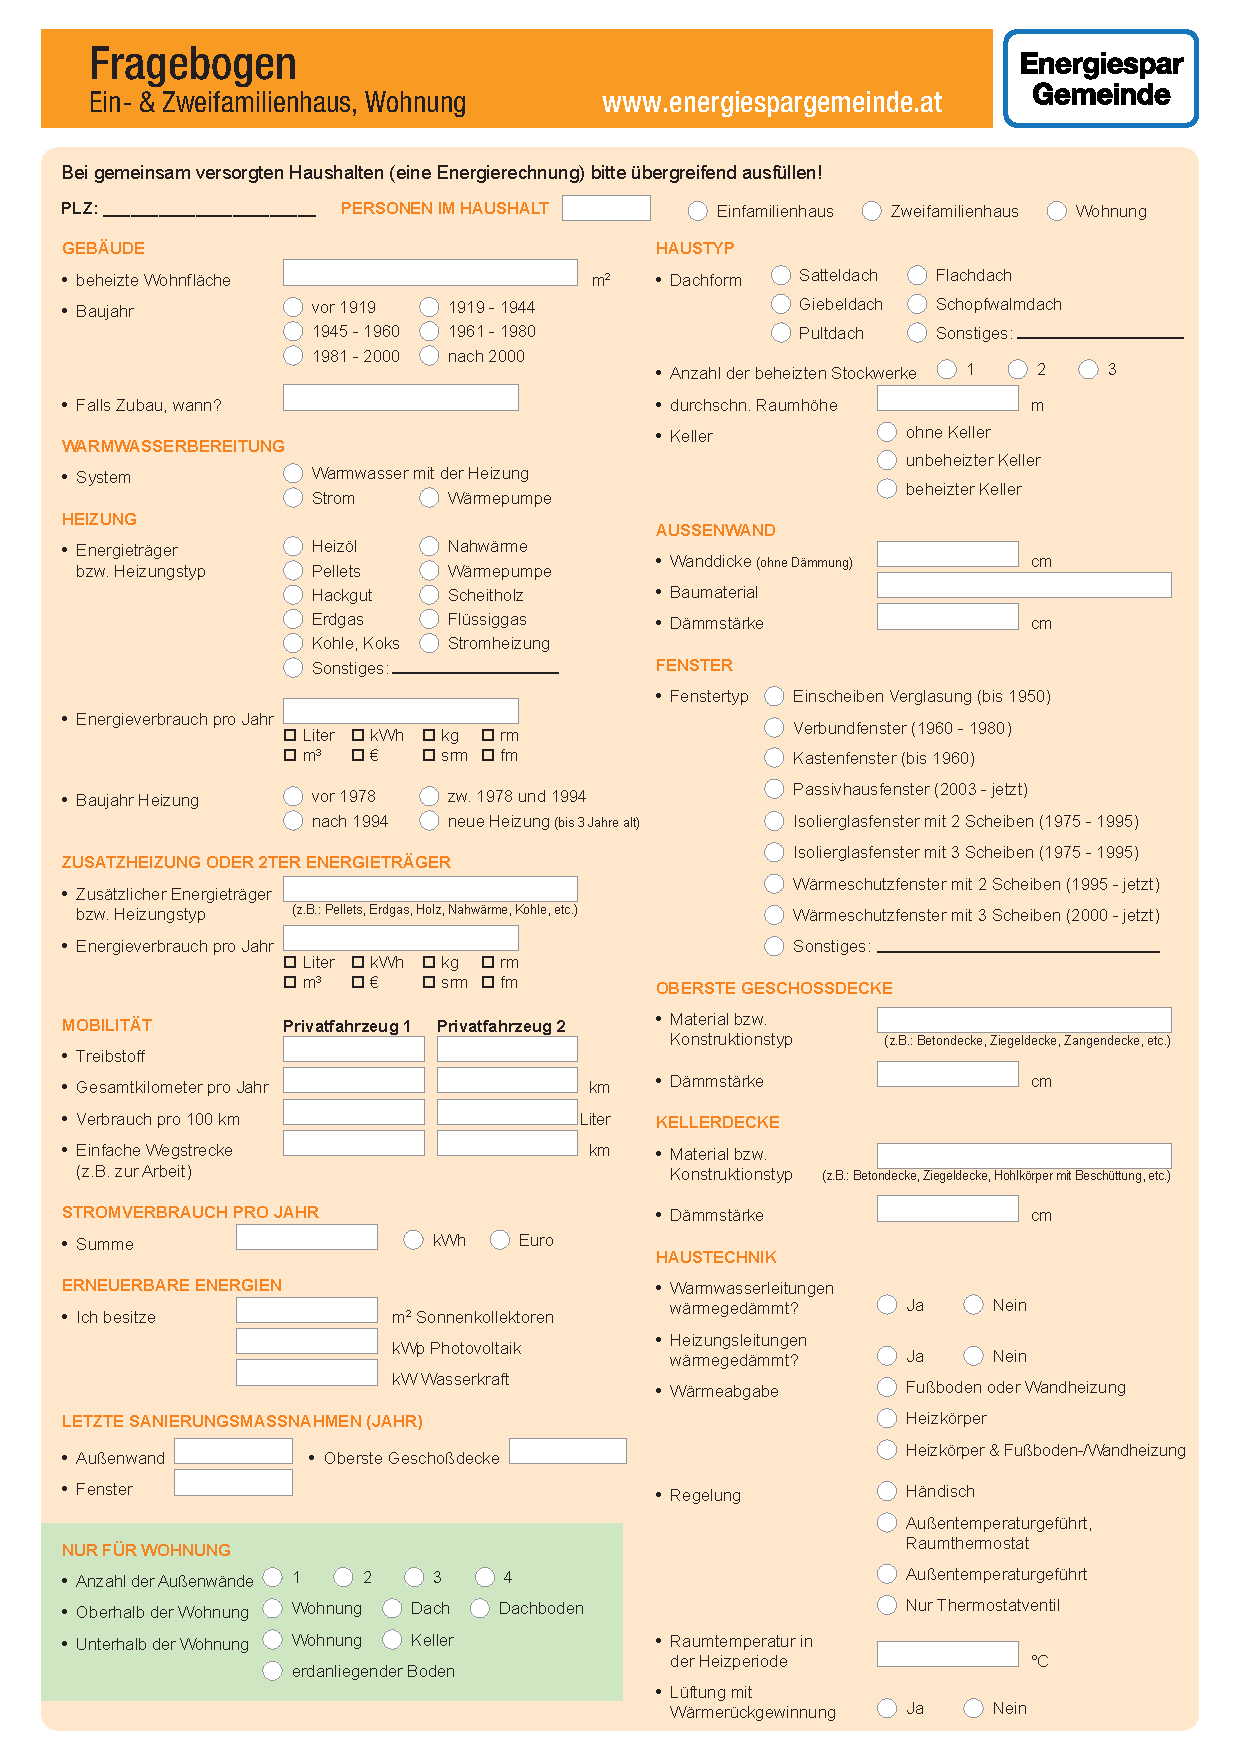
\includepdf[pages=1-,width=\textwidth,frame=true,pagecommand={}]{images/fragebogen}
\end{LaTeXCode}
%
Die eingebundenen Seiten werden durch \verb!width=\textwidth! automatisch auf die Textbreite
des \latex-Dokuments skaliert und durch \verb!frame=true! mit einer Umrandung versehen.

Dieses Beispiel geht davon aus, dass das externe PDF-Dokument im A4-Seitenformat ist.
Bei anderen Formaten muss man die Skalierung möglicherweise "händisch" einstellen,
falls die Seiten zu hoch werden (\zB\ mit \verb!width=0.9\textwidth!).

Wichtig ist auch, dass bei dem externen PDF-Dokument alle verwendeten \emph{Schriften}
(Fonts) korrekt und vollständig \emph{eingebettet} sind, da ansonsten das von \latex erzeugte 
PDF-Dokument nicht unabhängig von der Systemumgebung ist!


\section{Verweise auf eingebundene PDF-Seiten}

Möchte man im Text auf bestimmte PDF-Seiten verweisen,
so ist es am Einfachsten, die Seiten einzeln zu importieren und jeweils
mit einem \emph{Label} zu versehen, wie in diesem Beispiel:
%
\begin{LaTeXCode}[numbers=none]
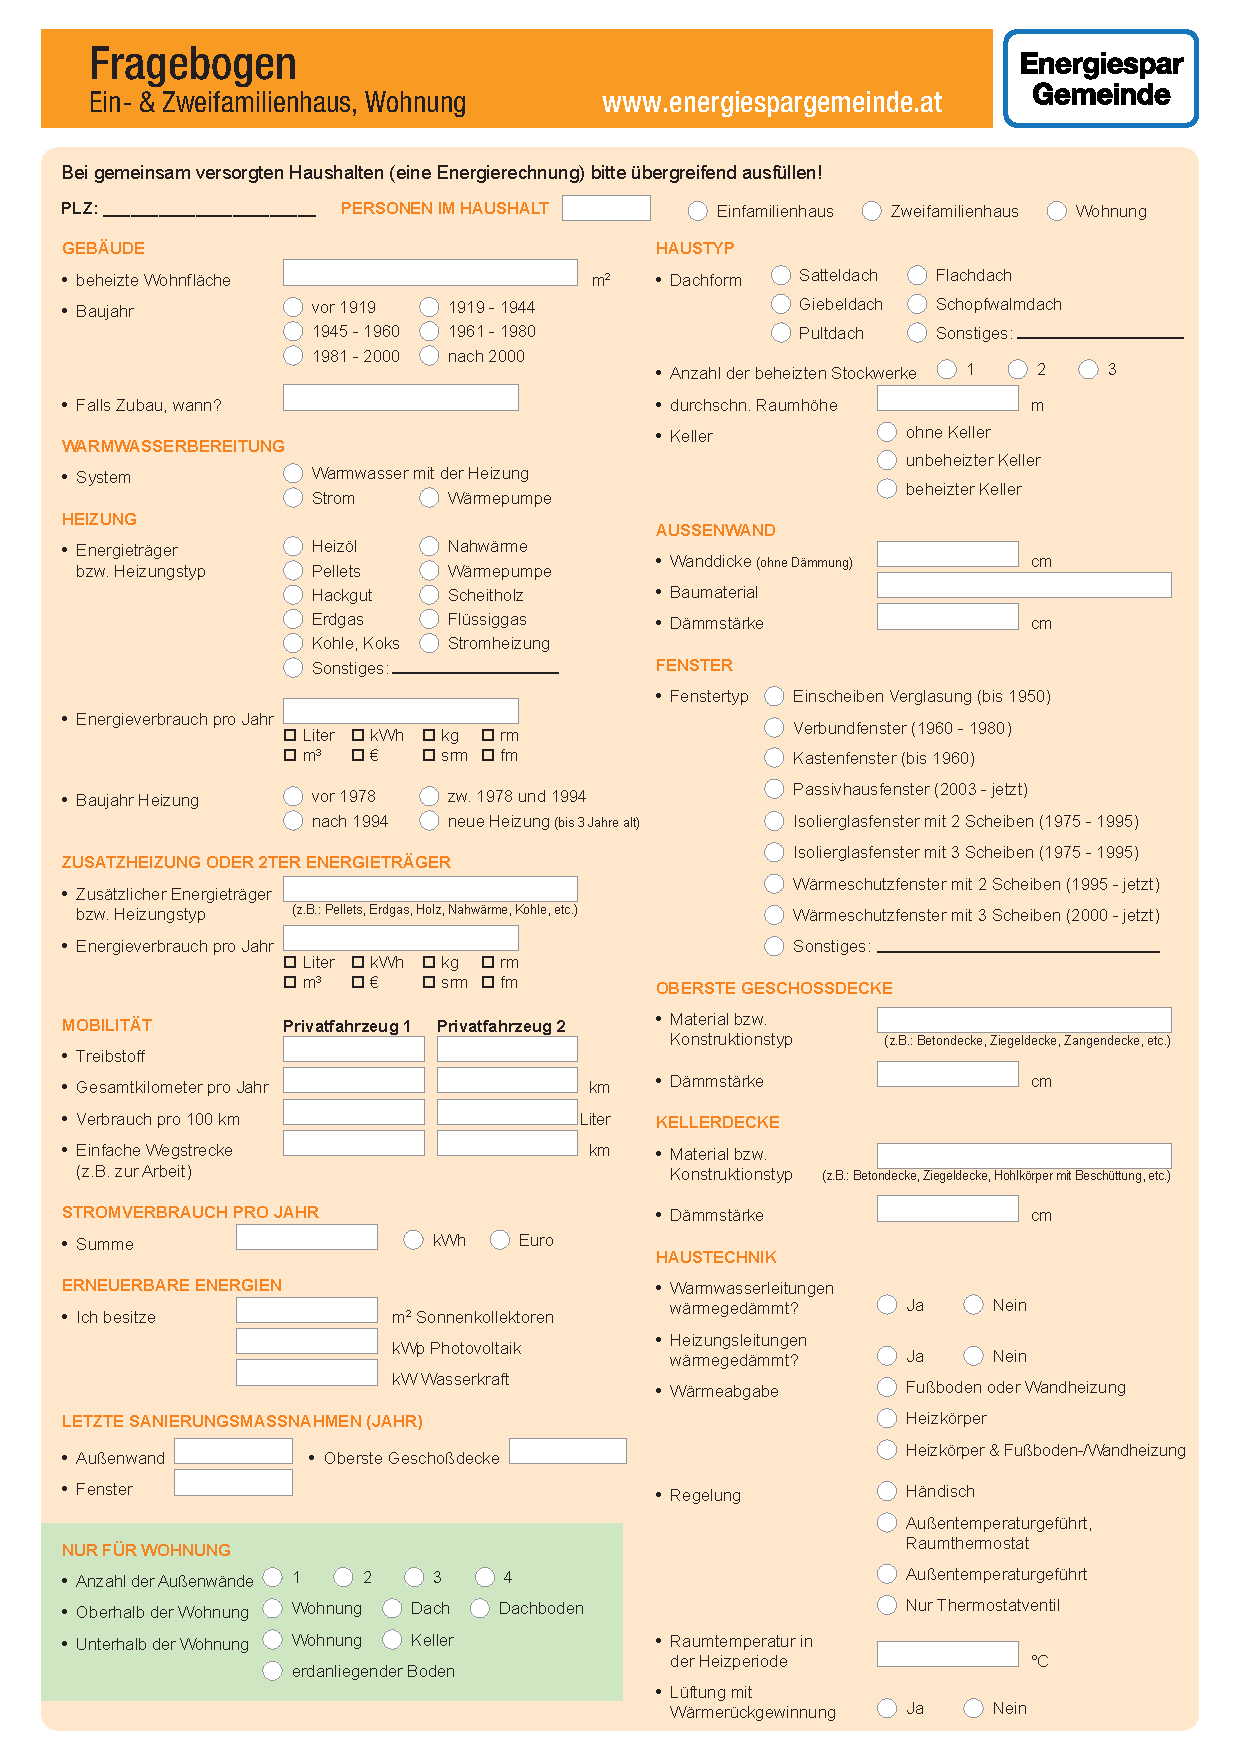
\includepdf[pages=1,width=\textwidth,frame=true,pagecommand={\label{PDF1}}]{images/fragebogen}
\includepdf[pages=2,width=\textwidth,frame=true,pagecommand={\label{PDF2}}]{images/fragebogen}
\end{LaTeXCode}
%
In diesem Fall könnte man beispielsweise mit \verb!\pageref{PDF2}!
die aktuelle Seitennummer der 2.\ Seite des eingebundenen PDF-Dokuments 
angeben.

Viele weitere Möglichkeiten (\zB\ die Angabe von Seitenintervallen) findet man
in der ausführlichen Dokumentation zum \texttt{pdfpages}-Paket.



% Und hiermit werden die PDF-Seiten tatsächlich eingebunden:
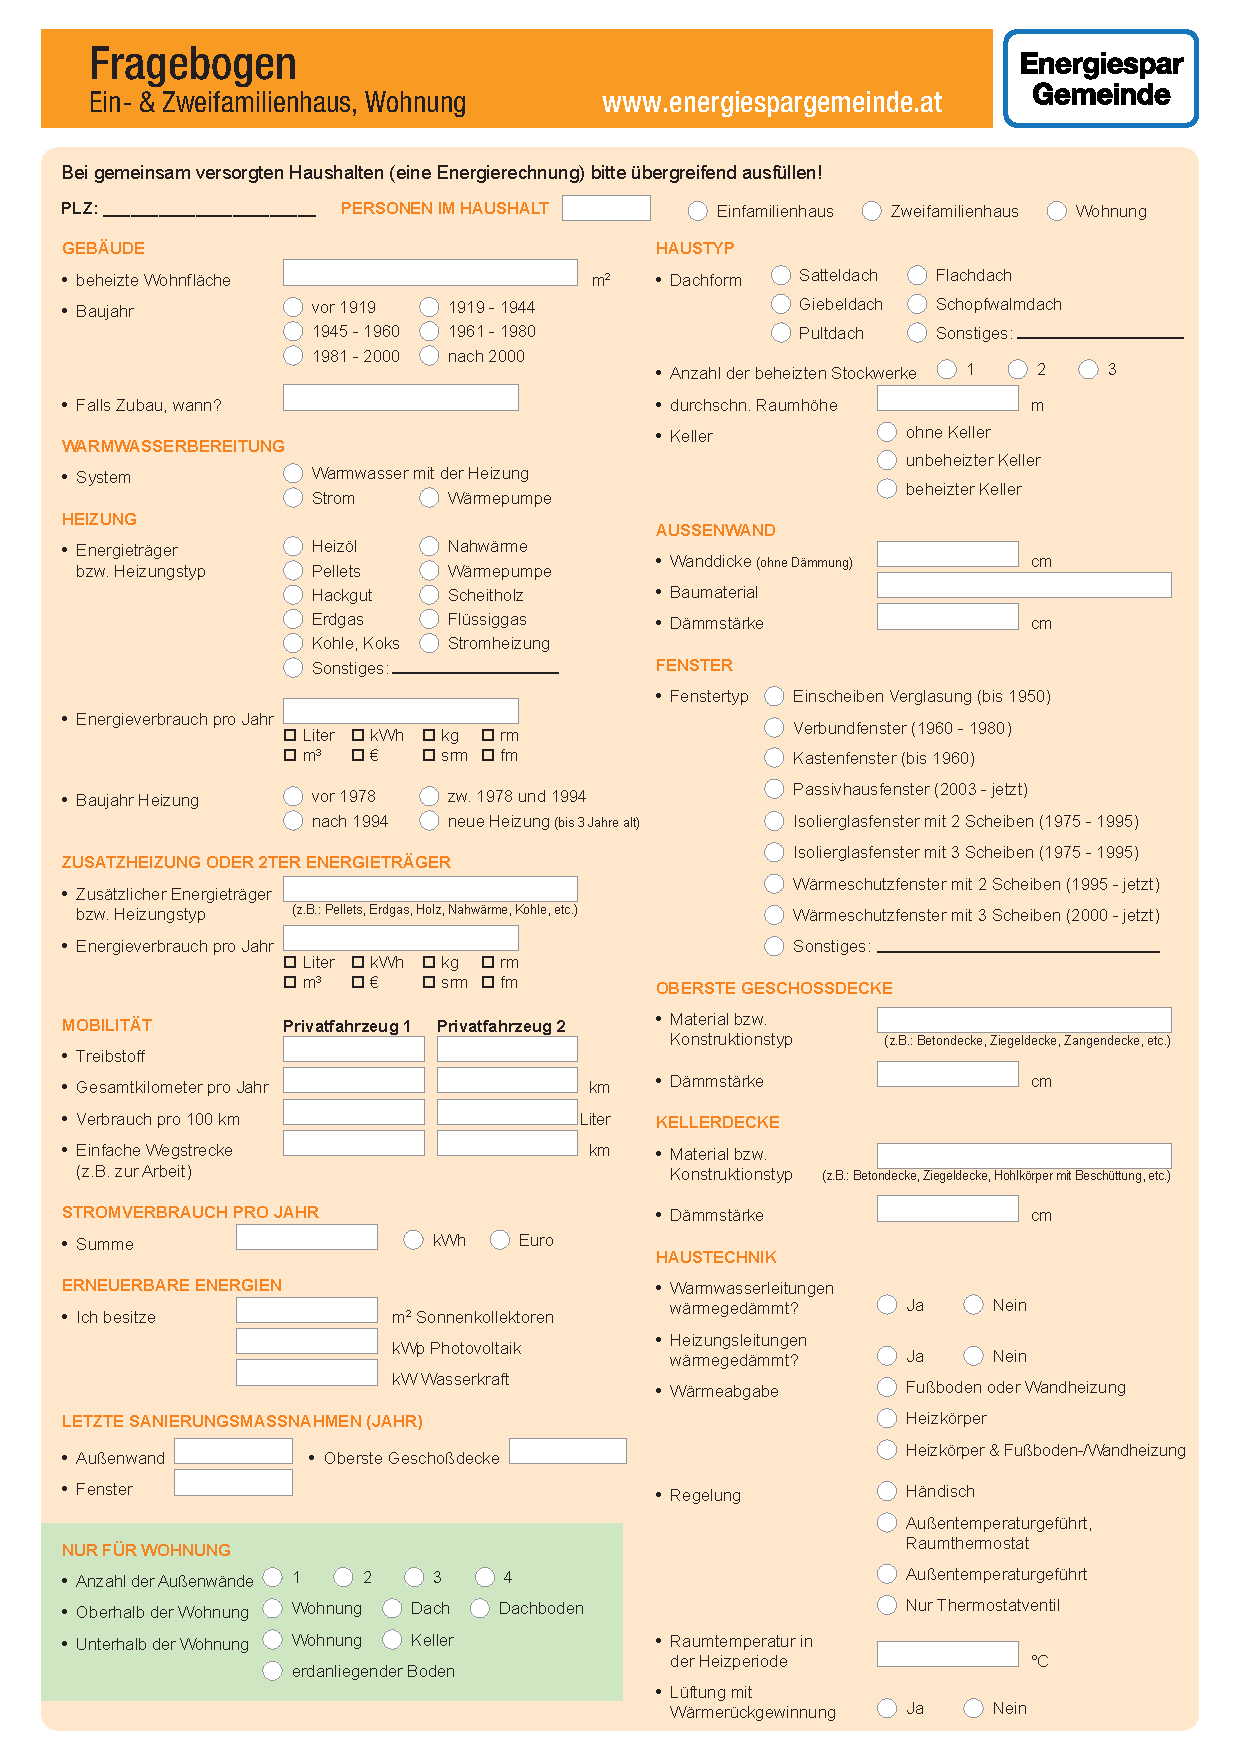
\includepdf[pages=1-,width=\textwidth,frame=true,pagecommand={}]{images/fragebogen}



